\section{Primzahlsuche}
\label{sec:Primzahlensuche}
\subsection{Langsam}
\label{subsec:langsameSuche}
Entsprechend der Aufgabenstellung wurde die Standard Primzahlensuche aus der Vorlesung implementiert.
In Tabelle \ref{tab: langsame Suche} ist der benötigte Aufwand T zu einer bestimmten Problemgröße N eingetragen.
In Abbildung \ref{fig:langsameSuche} ist T in Abhängigkeit zu N aufgetragen. Aus dieser ist zu entnehmen, dass das Steigungsverhalten exponentiell ist.
\begin{table}[htbp]
\caption{Langsame Primzahlensuche}
\label{tab: langsame Suche}
\centering
\begin{tabular}{l|r}
Problemgröße: N	&	Aufwand: T(N)	\\
\hline
100				&	9004			\\
200				&	39204			\\
300				&	88804			\\
400				&	158404			\\
500				&	248004			\\
\end{tabular}
\end{table}

\begin{figure}[htbp]
\centering
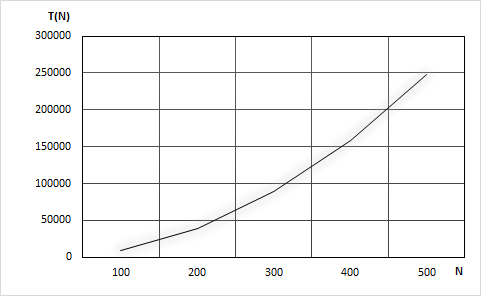
\includegraphics[scale=1.2]{LangsameSuche.png}
\caption{Langsame Primzahlensuche T(N)}
\label{fig:langsameSuche}
\end{figure}

\subsection{Schnelle}
\label{subsec:schnelleSuche}
Entsprechend der Aufgabenstellung wurde ein optimierte Primzahlensuche von der in Abschnitt \ref{subsec:langsameSuche} implementierten Suche implementiert.
In Tabelle \ref{tab:schnelleSuche} ist der benötigte Aufwand T zu einer bestimmten Problemgröße N eingetragen.
In Abbildung \ref{fig:langsameSuche} ist T in Abhängigkeit zu N aufgetragen. Aus dieser ist zu entnehmen, dass das Steigungsverhalten annähernd linear ist.
\begin{table}[htbp]
\caption{Schnelle Primzahlensuche}
\label{tab:schnelleSuche}
\centering
\begin{tabular}{l|r}
Problemgröße: N	&	Aufwand: T(N)	\\
\hline
100				&	235			\\
200				&	627			\\
300				&	1066		\\
400				&	1558		\\
500				&	2112		\\
\end{tabular}
\end{table}

\begin{figure}[htbp]
\centering
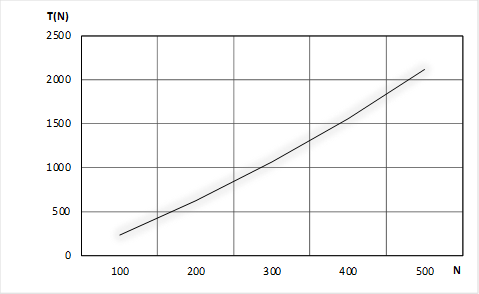
\includegraphics[scale=1.2]{SchnelleSuche.png}
\caption{Schnelle Primzahlensuche T(N)}
\label{fig:schnelleSuche}
\end{figure}


\subsection{Sieb des Eratosthenes}
\label{subsec:SiebSuche}
Entsprechend der Aufgabenstellung wurde die Suche nach dem 'Sieb des Eratosthenes' implementiert.
In Tabelle \ref{tab:siebSuche} ist der benötigte Aufwand T zu einer bestimmten Problemgröße N eingetragen.
In Abbildung \ref{fig:siebSuche} ist T in Abhängigkeit zu N aufgetragen. Aus dieser ist zu entnehmen, dass das Steigungsverhalten annähernd linear ist. \\
In Abbildung \ref{fig:vergleich} sind die Schnelle Suche und das Sieb des Eratosthenes im Vergleich zueinander zu sehen um die Unterschiede zu verdeutlichen.


\begin{table}[htbp]
\caption{Sieb des Eratosthenes}
\label{tab:siebSuche}
\centering
\begin{tabular}{l|r}
Problemgröße: N	&	Aufwand: T(N)	\\
\hline
100				&	182			\\
200				&	434			\\
300				&	712			\\
400				&	1015		\\
500				&	1316		\\
\end{tabular}
\end{table}

\begin{figure}[htbp]
\centering
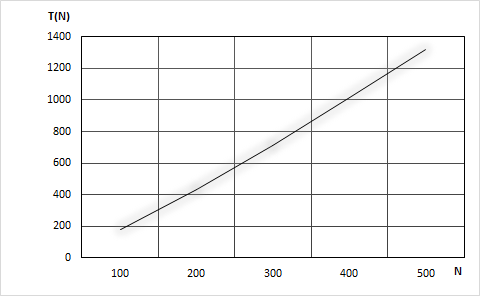
\includegraphics[scale=1.2]{SiebSuche.png}
\caption{Sieb des Eratosthenes T(N)}
\label{fig:siebSuche}
\end{figure}

\begin{figure}[htbp]
\centering
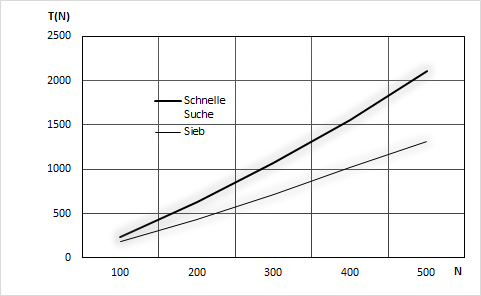
\includegraphics[scale=1.2]{SiebSchnellVergleich.png}
\caption{Schnelle Suche und Sieb des Eratosthenes im Vergleich T(N)}
\label{fig:vergleich}
\end{figure}

\subsection{Primzahleigenschaft feststellen}
\label{subsec:PrimFeststellen}

Entsprechend der Aufgabenstellung wurde eine Funktion zum Feststellen der Primzahleneigenschaft implementiert. Der Verlauf einer einzelnen Suche in diesem Algorithmus ist recht linear ohne Steigung, da ab dem ersten gefunden Teiler abgebrochen wird, weil die Primzahleigenschaft dann schon widerlegt ist. Ausreißer treten hauptsächlich bei Primzahlen auf oder wenn der erste Teiler gegen Ende des Prüfintervalls kommt. Aus diesem Grund wurde sich für eine Darstellung des Aufwandes um eine Primzahl entschieden, um das Verhältnis eines Ausreißers zu den Normalen Werten zu verdeutlichen. 
In Tabelle \ref{tab:Primeigenschaft} und Abbildung \ref{fig:Primeigenschaft} sind der Aufwand T in Abhängigkeit von der Zahl N (Problemgröße) abgebildet. Es wurde das Intervall von [500;506] gewählt welches die Primzahl 503 enthält.


\begin{table}[htbp]
\caption{Funktion zu Feststellung der Primzahleneigenschaft}
\label{tab:Primeigenschaft}
\centering
\begin{tabular}{l|r}
Problemgröße: N	&	Aufwand: T(N)	\\
\hline
500				&	1			\\
501				&	2			\\
502				&	1			\\
503				&	21			\\
504				&	1			\\
505				&	4			\\
506				&	1			\\
\end{tabular}
\end{table}

\begin{figure}[htbp]
\centering
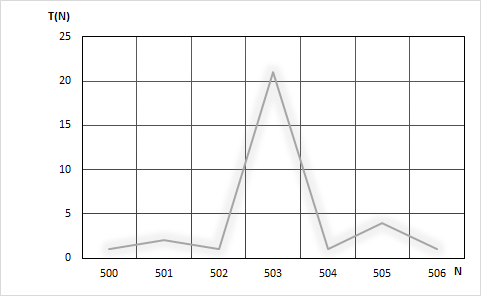
\includegraphics[scale=1.2]{PrimEigenschaft.png}
\caption{Feststellen der Primzahleneigenschaft T(N)}
\label{fig:Primeigenschaft}
\end{figure}